\documentclass[a4paper,12pt]{article} % only 10 (default), 11 and 12 pt are available

% NECESSARY PACKAGES
\usepackage[utf8]{inputenc} % to be able to use non-English characters
\usepackage{amsmath}  % improve math presentation
\usepackage{physics}
\usepackage{amssymb}
\usepackage{xcolor}
\usepackage{float}
\usepackage{caption} % captioning package of wonders
\usepackage{url} % to incorporate clickable links
\usepackage{cite} % takes care of citations
\usepackage[final]{hyperref} % adds hyper links inside the generated PDF file

% NECESSARY FOR INCREASED CUSTOMIZATION PACKAGES
\usepackage{newfloat} % for defining new float in environments (e.g: figure and tables are floats)
\usepackage{graphicx} % takes care of graphic including machinery
\usepackage{tabularx} % extra features for tabular environment
\usepackage{array} % provides 'programmable' tables (cells can be tweaked much more)
\usepackage[export]{adjustbox} % to include boxed content other than figures (e.g: boxed equations)
\usepackage{wrapfig} % to make figures wrap around text
\usepackage{subcaption} % to make sub-figures inside of figures
\usepackage[spanish]{babel}
% TWEAKS FOR PACKAGES
\usepackage[margin=2cm,a4paper]{geometry} % tweaks margins
\captionsetup{justification=centering} % caption justification
\captionsetup{font=small} % caption text size
\captionsetup{labelfont=bf} % caption label font emphasis (e.g: 'Figure X:')
\numberwithin{equation}{section} % equations are named according to their section (e.g: 2.1)
\numberwithin{figure}{section} % figures are named according to their section (e.g: 3.4)
\hypersetup{
    colorlinks=true,      % false: boxed links; true: colored links
    linkcolor=black,      % color of internal links
    citecolor=blue,       % color of links to bibliography
    filecolor=magenta,    % color of file links
    urlcolor=red          % color of website links
}

\usepackage{lipsum} % DELETE THIS AND BELOW \lipsum[]'s AND YOU'RE GOOD TO GO

%++++++++++++++++++++++++++++++++++++++++++++++++++++++++++++++++++++++++++++++++

% HERE GOES THE COVER PAGE SETUP
%\newcommand{\hwcourse}{\text{Astrofísica Extragaláctica y Cosmología}} % Title of your document
\newcommand{\hwnumber}{\text{Diplomado Sismología} \\ \text{Uso de Datos Sismológicos}} % Name of your study number
\newcommand{\hwname}{\text{Actividad 2: Localización y Cálculo de Magnitudes Seisan}} % Name of your study name
\newcommand{\hwdetails}{ \text{Informe de resultados obtenidos} \\ 
                            \text{Tarea 2} \\ % Details about your study
                            \\\text{ }\\
                            \text{\textit{Red Sismológica Nacional de Colombia - Dirección de Geoamenazas}} }
%\newcommand{\hwdate}{\text{In case you want to add a date other than submission date}}
\newcommand{\hwauthor}{Keneth Garcia} % Your name or your group's names
\newcommand{\HRule}{\rule{\linewidth}{0.5mm}} % line widths in the cover page

%++++++++++++++++++++++++++++++++++++++++++++++++++++++++++++++++++++++++++++++++

\begin{document}

% COVER PAGE IS COMPILED HERE
\begin{titlepage}
\begin{center} % Center remainder of the page
% LOGO SECTION

\includegraphics[width = 8cm]{Figures/sgc_logo}
\\[3cm]

% HEADING SECTIONS
\textsc{\LARGE Servicio Geológico Colombiano}\\[.5cm]
\textsc{\Large Universidad de Chile}\\[1.5cm]

% TITLE SECTION
\HRule \\[0.4cm]
%{ \huge \bfseries \hwcourse}\\ \vspace{.5cm} 
{ \huge \bfseries \hwnumber}\\ \vspace{.5cm} 
{ \large \bfseries \hwname}\\ \vspace{.5cm} 
{ \hwdetails}\\ \vspace{.5cm}
%{ \bfseries \hwdate}\\ \vspace{.5cm} 
\HRule \\[1.5cm]
\end{center} 

% AUTHOR SECTION
\begin{flushleft} % left oriented author section
    \large 
    \textit{Escrito por:}\\
    \hwauthor% Your name
\end{flushleft}
\vspace{5cm}
\makeatletter
Fecha: \today % \@date 
\vfill % Fill the rest of the page with white space
\makeatother
\end{titlepage}

%++++++++++++++++++++++++++++++++++++++++++++++++++++++++++++++++++++++++++++++++

\newpage

%\tableofcontents

%\newpage

%\begin{abstract}
    %\lipsum[1]
%\end{abstract}

%\newpage

\section{Introducción}

La localización precisa de los sismos y la determinación de sus mecanismos focales constituyen herramientas fundamentales para el estudio de la sismicidad y la interpretación de los procesos tectónicos que la generan. A partir de los tiempos de arribo de las ondas sísmicas registradas en una red de estaciones, es posible estimar la ubicación del hipocentro, su profundidad y el tiempo de origen de un evento. De manera complementaria, el análisis de las polaridades de las primeras llegadas de ondas P permite restringir la geometría de la falla y el sentido del movimiento que produjo la ruptura, aportando información esencial para clasificar el tipo de sismo y relacionarlo con el contexto tectónico regional.

En esta actividad se empleará el programa SEISAN para procesar registros sísmicos en formato \textit{miniSEED} asociados a eventos ocurridos en Chile durante los años 2021 y 2022. El procesamiento comprende la visualización de las formas de onda, la identificación y el picado de los arribos de las fases P y S, y el registro de la polaridad de la primera llegada de la onda P en la componente vertical. A partir de estas observaciones se realizará la localización de dos eventos seleccionados, procurando obtener soluciones con un error cuadrático medio (\textit{RMS}) inferior a $0{,}5$~s y una cobertura azimutal adecuada de las estaciones.

La estimación de las localizaciones dependerá de la comparación entre los tiempos de viaje observados y aquellos calculados mediante un modelo de velocidades predefinido por el material suplementario. Por ello, las diferencias entre ambos conjuntos de tiempos constituyen una forma de analizar las incertidumbres en el picado de fases, las limitaciones de la cobertura instrumental o aquellas simplificaciones inherentes al modelo de velocidades utilizado para representar la estructura del margen de subducción chileno. La evaluación de dichos factores permitirá discutir la calidad y las limitaciones de cada solución hipocentral.

Asimismo, los mecanismos focales serán calculados mediante los programas \texttt{FPFIT} y \texttt{FOCMEC}, utilizando las polaridades de las primeras llegadas de ondas P. Como veremos más adelante, la comparación entre ambos métodos permitirá evaluar el nivel de restricción proporcionado por las observaciones disponibles, identificar posibles ambigüedades en las soluciones y analizar las diferencias que puedan surgir debido a los criterios de búsqueda y ajuste empleados por cada programa.

Finalmente, las localizaciones y los mecanismos focales obtenidos serán comparados con información reportada por agencias sismológicas y, cuando estén disponibles, con resultados publicados en literatura científica. Esta comparación permitirá evaluar la coherencia de los resultados alcanzados y discutir la clasificación tectónica de cada sismo a partir de su posición en planta, profundidad, mecanismo focal y relación con las principales estructuras activas del territorio chileno.

El presente documento presenta los resultados obtenidos durante el desarrollo de la actividad. Inicialmente, se describen los procedimientos aplicados en SEISAN para el procesamiento de las formas de onda, el picado de fases, la localización hipocentral y el cálculo de mecanismos focales. A continuación, se presentan y discuten las localizaciones, los mecanismos focales, la cobertura de estaciones, la comparación con soluciones de agencias sismológicas o literatura científica y la interpretación tectónica de los eventos analizados. Finalmente, se sintetizan los principales hallazgos, las limitaciones identificadas y la coherencia general de las soluciones obtenidas.

\newpage

\section{Metodología}

\subsection{Instalación y configuración de SEISAN}

El procesamiento de los eventos se realizó mediante el programa \texttt{SEISAN} en un sistema operativo Windows. La instalación se efectuó a partir del instalador oficial para Windows, utilizando la configuración predeterminada y la estructura de directorios propuesta por el programa, con el directorio principal ubicado en \texttt{C:\textbackslash Seismo}. Esta instalación crea las carpetas necesarias para almacenar datos de formas de onda, archivos de eventos, configuraciones y programas ejecutables, entre las que se encuentran \texttt{WAV}, \texttt{REA}, \texttt{DAT}, \texttt{COM} y \texttt{PRO}.

Para garantizar la ejecución de los comandos de SEISAN desde la consola de Windows, se verificó la configuración de las variables de entorno y de las rutas requeridas. En particular, se configuró la variable \texttt{SEISAN\_TOP} para que apuntara al directorio de instalación principal y se incluyeron las carpetas \texttt{COM} y \texttt{PRO} dentro de la variable \texttt{PATH} del sistema. Esta configuración permite que los programas de localización, visualización y cálculo de mecanismos focales reconozcan la estructura interna del software y puedan ejecutarse desde la ventana de comandos \cite{seisan_windows_manual}.

Posteriormente, los archivos de formas de onda en formato \textit{miniSEED} fueron ubicados en el directorio \texttt{C:\textbackslash Seismo\textbackslash WAV}. Asimismo, se creó una base de datos de trabajo dentro de \texttt{C:\textbackslash Seismo\textbackslash REA}, organizada mediante un directorio de cinco letras mayúsculas y subdirectorios correspondientes al año y mes de ocurrencia de cada evento. Los archivos \textit{S-file} fueron ubicados en sus directorios temporales respectivos, mientras que el archivo \texttt{STATION0.HYP}, que contiene las coordenadas de las estaciones y el modelo de velocidades, se instaló en \texttt{C:\textbackslash Seismo\textbackslash DAT}, reemplazando la configuración predeterminada.

\subsection{Selección de eventos}

De los tres eventos suministrados para la actividad, se seleccionaron los registros denominados \texttt{event20210523T215859} y \texttt{event20221210T072548}. Esta selección permitió trabajar con dos eventos ocurridos en años distintos, registrados por estaciones de las redes C1 y CX, y comparar sus localizaciones y mecanismos focales dentro del contexto sismotectónico chileno.

El primer evento corresponde a un sismo ocurrido el 23 de mayo de 2021 a las 21:58:59 UTC, mientras que el segundo corresponde a un evento ocurrido el 10 de diciembre de 2022 a las 07:25:48 UTC. La información de referencia de ambos eventos fue consultada en la base de datos pública del Centro Sismológico Nacional (CSN), utilizando la fecha y hora de origen como criterios de búsqueda~\cite{csn_event_database}. Para cada evento se recopiló, de forma resumida, la fecha y hora de ocurrencia, la localización geográfica, la profundidad, la magnitud reportada y la descripción espacial de referencia proporcionada por el CSN. Estos antecedentes se utilizarán posteriormente para comparar las localizaciones obtenidas mediante SEISAN con las soluciones institucionales disponibles.

\subsection{Preparación y visualización de las trazas}

Una vez organizada la base de datos, se inició la interfaz de eventos de SEISAN mediante el comando \texttt{eev}, especificando el año, el mes y el nombre de la base de datos creada. Desde la lista de eventos se utilizó el comando \texttt{po} para abrir las formas de onda asociadas a cada \textit{S-file}. La visualización permitió revisar los registros de las estaciones disponibles, sus componentes y la calidad general de la señal.

Durante esta etapa se inspeccionaron las trazas para identificar las estaciones con relaciones señal--ruido adecuadas y ventanas temporales que permitieran reconocer de manera confiable los arribos de las fases sísmicas. Cuando fue necesario, se ajustó la escala temporal y de amplitud para mejorar la visualización de los primeros arribos, y se aplicaron filtros de frecuencia únicamente cuando estos facilitaron la identificación de fases sin alterar de forma significativa la señal observada.

\subsection{Picado de fases y polaridades}

Para cada estación con señal utilizable se identificaron y marcaron los tiempos de llegada de las ondas P y S. En SEISAN, las fases P fueron registradas como impulsivas o emergentes según la nitidez de su inicio; de manera análoga, las fases S se clasificaron de acuerdo con la claridad de su llegada. Se priorizó el uso de fases P y S en las estaciones con señales claras, aunque en algunos casos se registró únicamente una de las fases cuando la otra no podía identificarse con suficiente confianza.

Las llegadas P fueron marcadas como impulsivas mediante la opción \texttt{IP} o como emergentes mediante \texttt{EP}. Además, en la componente vertical de cada estación se registró la polaridad de la primera llegada P: una polaridad positiva o compresional fue asignada cuando el primer movimiento se dirigió hacia arriba, mientras que una polaridad negativa o dilatacional fue asignada cuando el primer movimiento se dirigió hacia abajo. Las observaciones con baja relación señal--ruido, ambigüedad en el arribo inicial o polaridad poco definida fueron descartadas para evitar que afectaran la localización y el cálculo del mecanismo focal.

Los tiempos de arribo P y S fueron utilizados posteriormente para obtener una solución hipocentral mediante el ajuste entre los tiempos observados y los tiempos teóricos calculados por SEISAN a partir del modelo de velocidades incluido en el archivo \texttt{STATION0.HYP}. Se buscó obtener soluciones con un error cuadrático medio, o \textit{RMS}, inferior a $0{,}5$~s, de acuerdo con el criterio definido para la actividad.

\subsection{Cálculo de mecanismos focales}

Los mecanismos focales fueron estimados a partir de las polaridades de las primeras llegadas de ondas P marcadas en las componentes verticales. Para este propósito se utilizaron los dos programas indicados en la actividad: \texttt{FPFIT} y \texttt{FOCMEC}. Ambos métodos emplean la distribución de polaridades compresionales y dilatacionales respecto de la localización del evento y las estaciones, con el fin de estimar las orientaciones de los planos nodales y el tipo de mecanismo de falla asociado.

En primer lugar, se ejecutó \texttt{FPFIT}, obteniendo una solución de mecanismo focal ajustada a las polaridades ingresadas. Posteriormente, se utilizó \texttt{FOCMEC}, el cual explora un conjunto de soluciones posibles a partir de diferentes combinaciones de \textit{strike}, \textit{dip} y deslizamiento. Durante la ejecución de \texttt{FOCMEC} se consideraron pesos relativos para reducir la influencia de observaciones próximas a los planos nodales y se realizaron pruebas con distintos valores de tolerancia para errores de polaridad e incrementos angulares de búsqueda.

Cuando \texttt{FOCMEC} entregó más de una solución admisible, la selección de la solución preferida se realizó considerando el menor número de polaridades incompatibles, la distribución azimutal de las estaciones, la coherencia con el mecanismo entregado por \texttt{FPFIT} y la consistencia con la localización y el contexto tectónico del evento. Finalmente, las soluciones obtenidas mediante ambos programas serán comparadas entre sí y con los mecanismos focales, localizaciones y parámetros publicados por el CSN u otras fuentes sismológicas disponibles.

\newpage

\section{Resultados}

\subsection{Evento del 23 de mayo de 2021}

\subsubsection{Selección de fases y polaridades}

\begin{figure}[]
    \centering

    \begin{subfigure}[b]{0.49\textwidth}
        \centering
        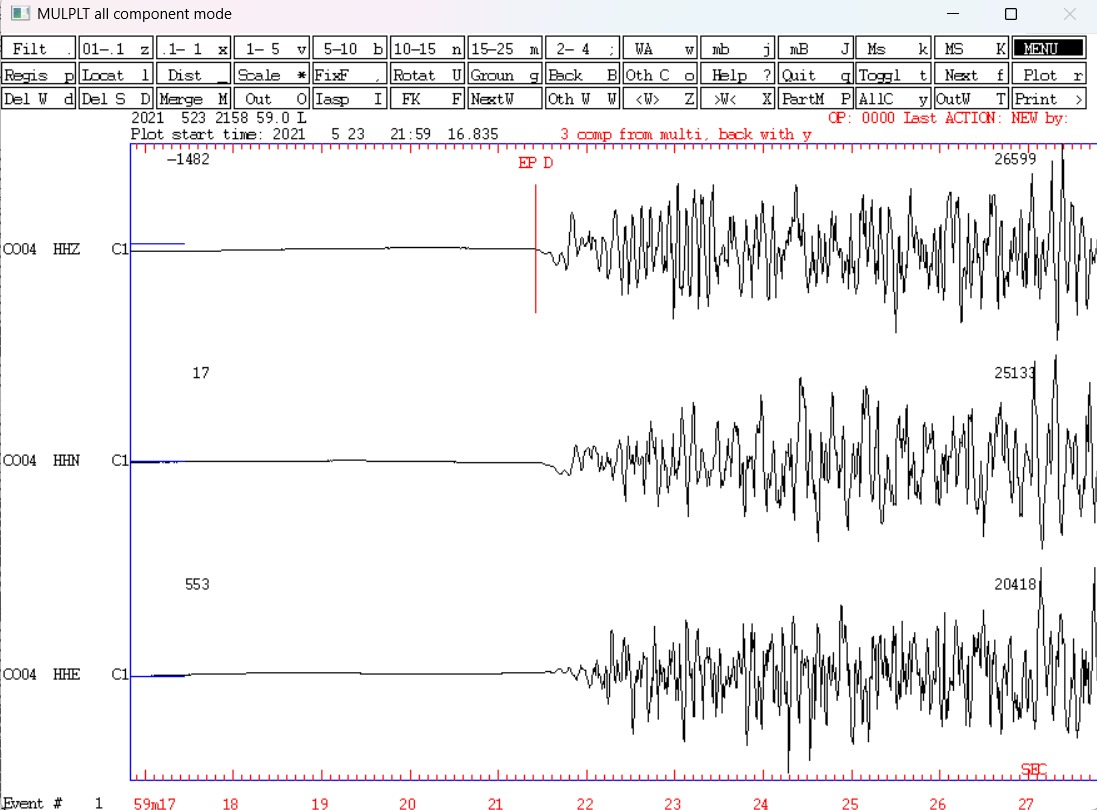
\includegraphics[width=\textwidth]{Figures/pick_ES_C004_20210523}
        \caption{Ejemplo de selección de una fase P emergente con polaridad dilatacional (\texttt{EPD}) en la estación \texttt{C004}, registrada en las componentes \texttt{HHZ}, \texttt{HHN} y \texttt{HHE}. La marca roja indica el instante seleccionado para el arribo de la fase P.}
        \label{fig:pick-es-c004-20210523}
    \end{subfigure}
    \hfill
    \begin{subfigure}[b]{0.49\textwidth}
        \centering
        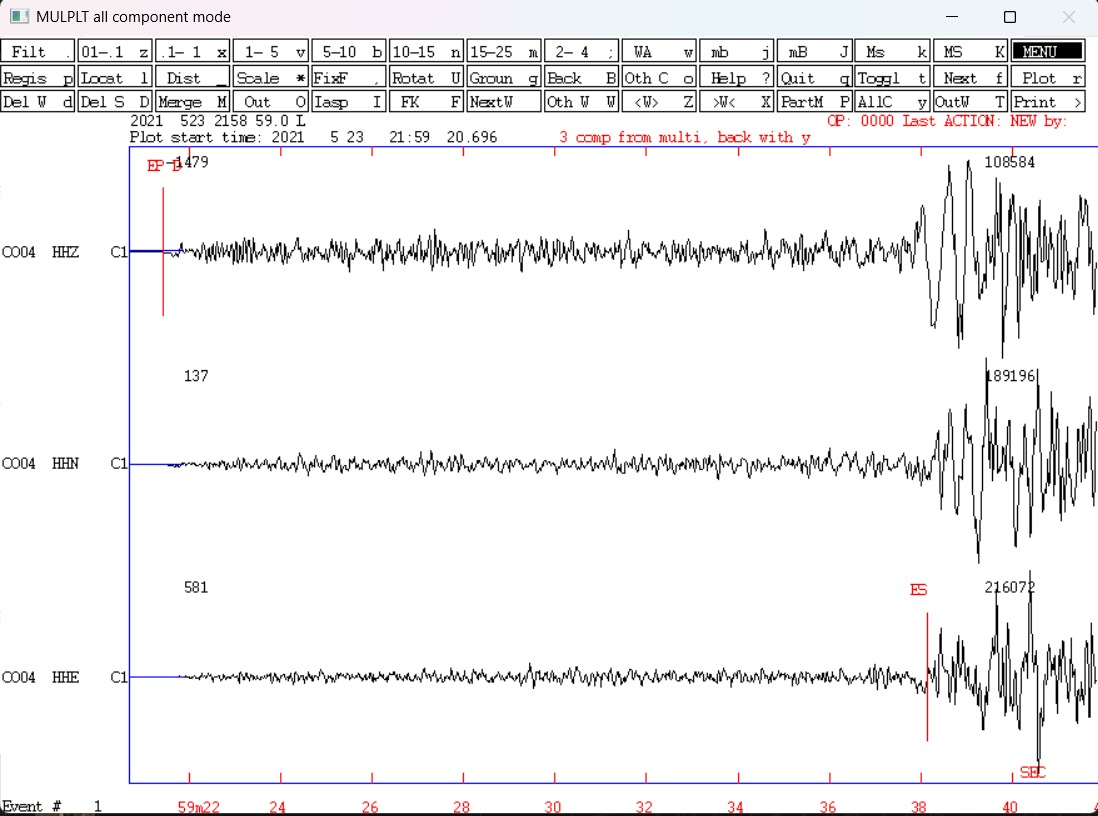
\includegraphics[width=\textwidth]{Figures/pick_EP_C004_20210523}
        \caption{Ejemplo de selección de una fase P emergente con polaridad dilatacional (\texttt{EP D}) y una fase S emergente (\texttt{ES}) en la estación \texttt{C004}. La marca roja indica el instante de llegada seleccionado para las fases.}
        \label{fig:pick-ep-c004-20210523}
    \end{subfigure}

    \caption{Ejemplos de selección manual de arribos de fases para el evento del 23 de mayo de 2021, visualizados en SEISAN. Las trazas corresponden a las componentes vertical y horizontales de la estación \texttt{C004} de la red \texttt{C1}.}
    \label{fig:picks-evento-20210523}
\end{figure}

El primer evento analizado corresponde al archivo \texttt{event20210523T215859}, cuya forma de onda fue revisada en SEISAN mediante la visualización de las tres componentes registradas por las estaciones disponibles. Para la localización del evento y el cálculo posterior del mecanismo focal, se identificaron los arribos de las fases P y S en los registros que presentaron una relación señal--ruido adecuada. Además, para las primeras llegadas P se registró su carácter impulsivo o emergente y, cuando fue posible identificarla con claridad, su polaridad en la componente vertical.

La Figura~\ref{fig:picks-evento-20210523} presenta dos ejemplos del proceso de selección de fases realizado para este evento en la estación \texttt{C004} de la red \texttt{C1}. En ambas subfiguras se muestran simultáneamente las componentes vertical (\texttt{HHZ}) y horizontales (\texttt{HHN} y \texttt{HHE}), lo que permitió comparar la respuesta de la señal entre componentes y reconocer los cambios de amplitud asociados a las llegadas sísmicas. Las líneas verticales rojas corresponden a las marcas realizadas durante el procesamiento en SEISAN.

En la Figura~\ref{fig:picks-evento-20210523}b se observa un ejemplo de una fase S emergente (\texttt{ES}) seleccionada en la componente \texttt{HHE}. El arribo se identificó a partir del incremento progresivo de amplitud de la señal, especialmente visible en las componentes horizontales. Por su parte, la Figura~\ref{fig:picks-evento-20210523}a presenta una fase P emergente con polaridad dilatacional (\texttt{EP D}) identificada en la componente vertical \texttt{HHZ}. Estas selecciones fueron incorporadas en el archivo del evento para su utilización posterior en la localización hipocentral y en el cálculo de las soluciones de mecanismo focal.

\begin{figure}[htbp]
    \centering

    \begin{subfigure}[b]{0.49\textwidth}
        \centering
        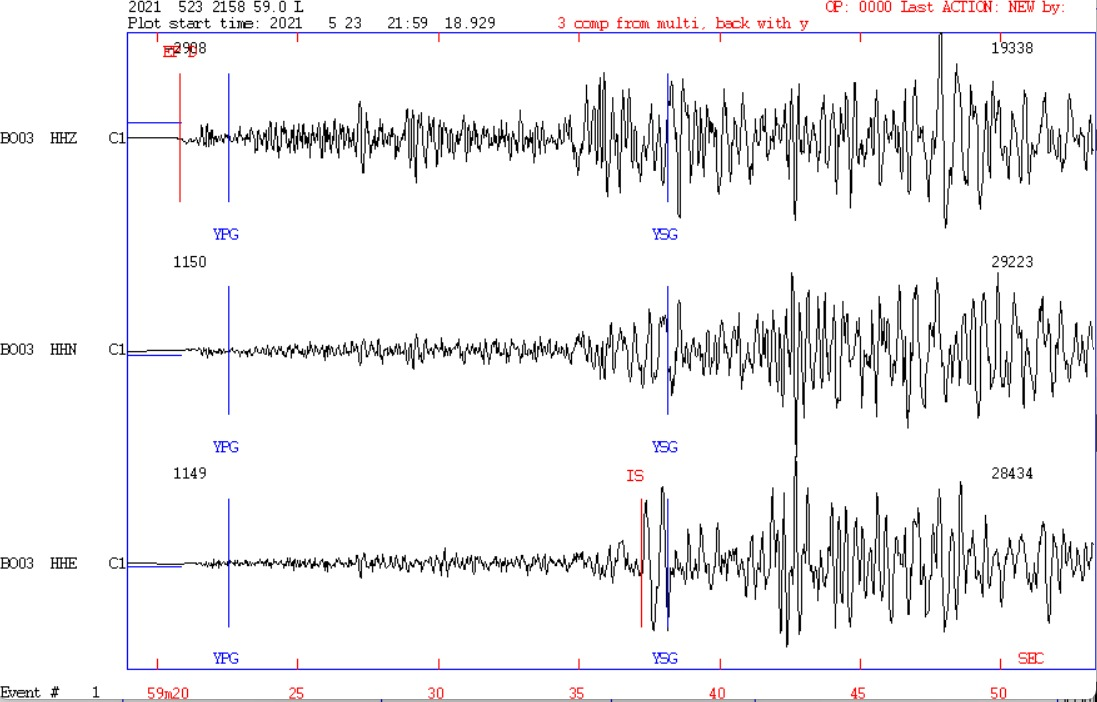
\includegraphics[width=\textwidth]{Figures/picks_observados_teoricos_B003_1_20210523}
        \caption{Comparación entre arribos observados y tiempos teóricos para la estación \texttt{B003}. Las marcas rojas representan los picks manuales; las líneas azules corresponden a los tiempos teóricos de las fases P y S calculados por SEISAN. Se aprecia una fase S impulsiva (\texttt{IS}) seleccionada en la componente \texttt{HHE}.}
        \label{fig:picks-teoricos-b003-1-20210523}
    \end{subfigure}
    \hfill
    \begin{subfigure}[b]{0.49\textwidth}
        \centering
        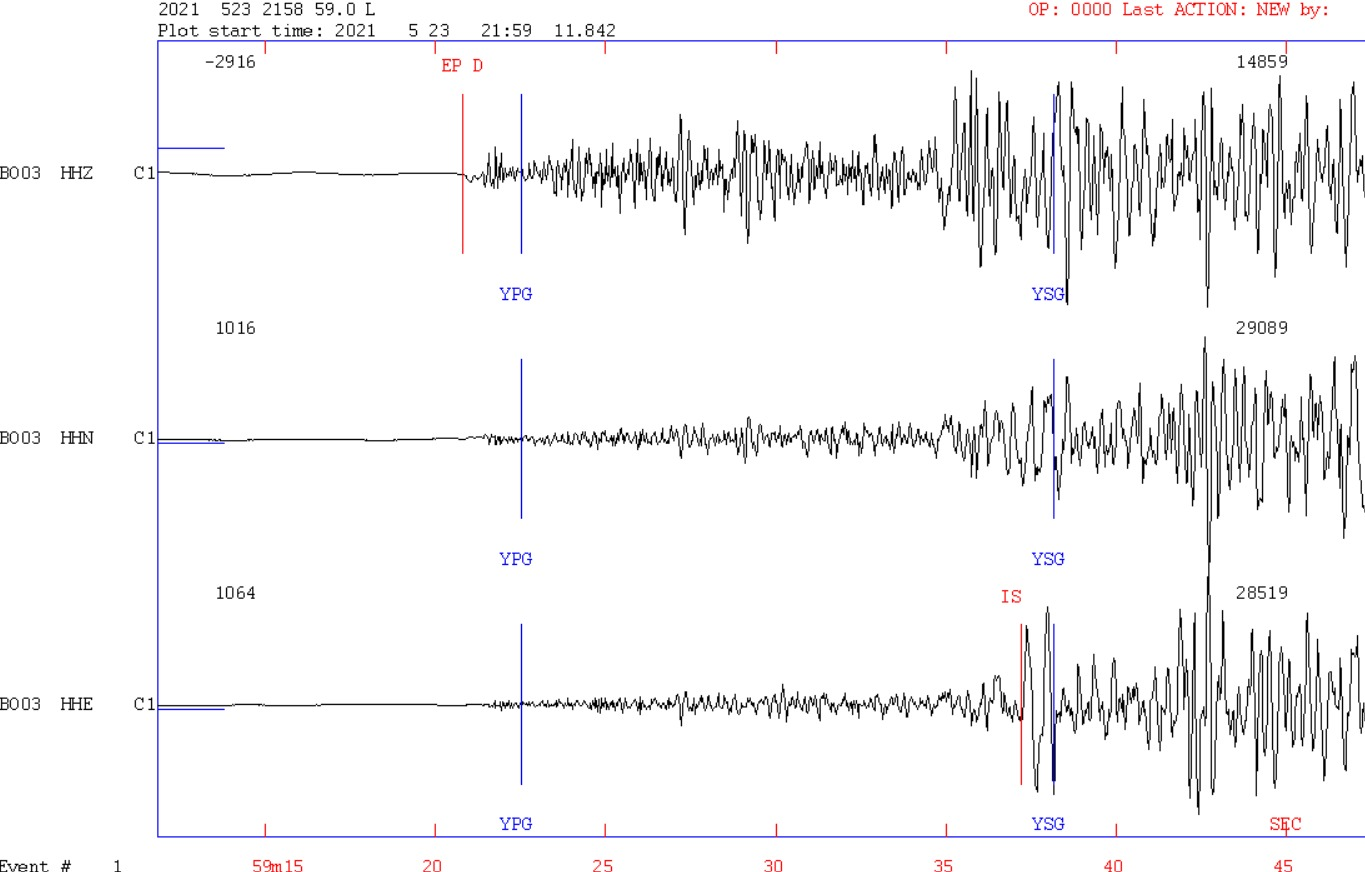
\includegraphics[width=\textwidth]{Figures/picks_observados_teoricos_B003_2_20210523}
        \caption{Comparación entre picks observados y teóricos en otra ventana temporal de la estación \texttt{B003}. Se muestra una fase P emergente con polaridad dilatacional (\texttt{EP D}) y una fase S impulsiva (\texttt{IS}), ambas marcadas en rojo; los indicadores azules corresponden a los arribos teóricos calculados para las fases P y S.}
        \label{fig:picks-teoricos-b003-2-20210523}
    \end{subfigure}

    \caption{Comparación entre los tiempos de llegada observados y los tiempos teóricos calculados por SEISAN para el evento del 23 de mayo de 2021. Las marcas rojas corresponden a los picks manuales, mientras que las marcas azules corresponden a las llegadas teóricas calculadas mediante el modelo de velocidades configurado.}
    \label{fig:picks-observados-teoricos-20210523}
\end{figure}

La Figura~\ref{fig:picks-observados-teoricos-20210523} presenta ejemplos de la comparación entre las fases seleccionadas manualmente en las trazas y los tiempos teóricos calculados por SEISAN luego de aplicar el modelo de velocidades configurado en el archivo \texttt{STATION0.HYP}. Las marcas rojas corresponden a los arribos observados e identificados durante el procesamiento manual, mientras que las líneas azules representan los tiempos teóricos de las fases P y S estimados por el programa para la solución de localización calculada.

En ambas subfiguras se observa que los picks teóricos no coinciden exactamente con los arribos seleccionados sobre la señal. Este desfase es esperable, ya que los tiempos teóricos son calculados a partir de un modelo de velocidades simplificado, mientras que los tiempos observados corresponden a la propagación real de las ondas a través de una estructura cortical y de subducción heterogénea. Además, pequeñas diferencias pueden originarse en la localización preliminar del evento, en la geometría entre el hipocentro y cada estación, en variaciones locales de velocidad y en la incertidumbre inherente a la identificación manual de fases, particularmente cuando los arribos son emergentes o presentan una relación señal--ruido limitada.

Por esta razón, los picks no deben desplazarse automáticamente hasta coincidir con las llegadas teóricas con el único propósito de disminuir el valor del \textit{RMS}. Los tiempos observados deben conservarse en el punto donde la señal muestra físicamente el inicio de la fase P o S, pues modificar las observaciones para forzar su ajuste al modelo introduce un sesgo artificial y elimina información sobre las discrepancias entre el modelo de velocidades y la estructura real del medio. El valor de \textit{RMS} debe utilizarse como un indicador de la calidad global de la localización y de la consistencia entre datos y modelo, pero siempre en conjunto con una revisión visual de la calidad de los picks y de la cobertura de estaciones.

\subsubsection{Localización hipocentral}

\begin{figure}[htbp]
    \centering
    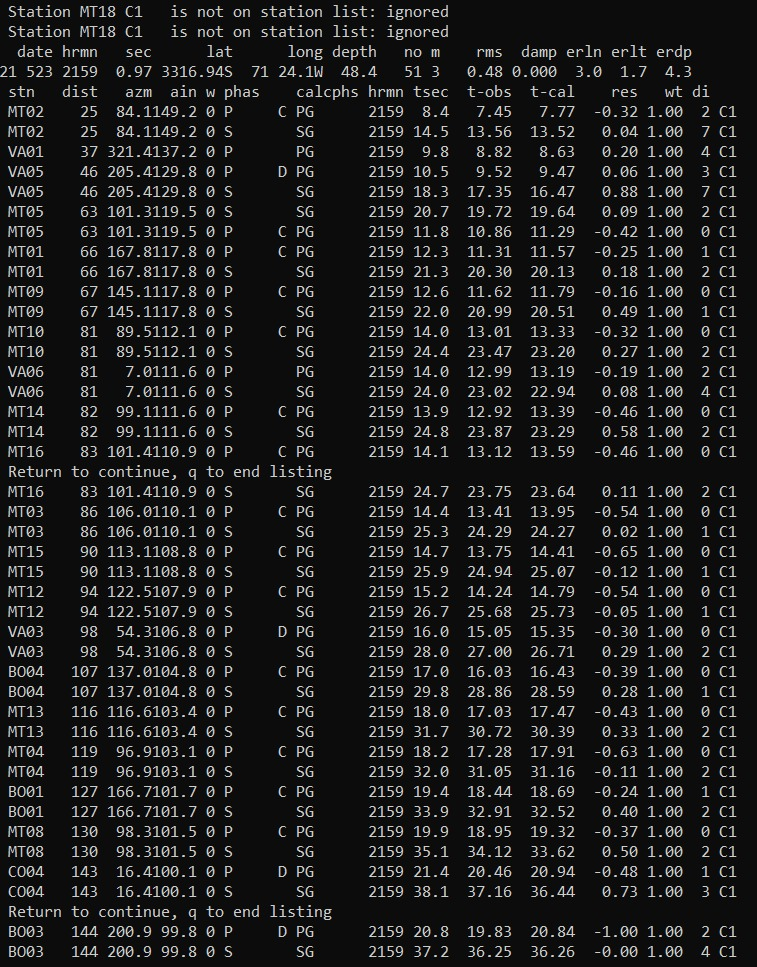
\includegraphics[width=0.80\textwidth]{Figures/RMS_1}
    \caption{Salida de SEISAN para la localización del evento del 23 de mayo de 2021. La figura presenta los parámetros de la solución hipocentral y las observaciones de fases P y S utilizadas en el ajuste. Para cada estación se muestran la distancia, el acimut, la fase observada, los tiempos de viaje observado y calculado, el residuo temporal y el peso asignado. La solución obtenida presenta un \textit{RMS} de $0{,}48$~s, calculado a partir de $51$ observaciones.}
    \label{fig:residuos-localizacion-20210523}
\end{figure}

La Figura~\ref{fig:residuos-localizacion-20210523} muestra la salida numérica generada por SEISAN después de ejecutar la localización del evento del 23 de mayo de 2021. Esta salida resume los parámetros de la solución hipocentral obtenida mediante el modelo de velocidades configurado y presenta, para cada estación y fase seleccionada, la comparación entre los tiempos de arribo observados y los tiempos teóricos calculados.

La cabecera de la salida indica una solución localizada aproximadamente a $33{,}16^\circ$S y $71{,}24^\circ$W, con una profundidad de $48{,}4$~km. Asimismo, se reportan $51$ observaciones utilizadas en el ajuste y un valor de amortiguamiento igual a $0{,}000$. El modelo utilizó observaciones de fases P y S registradas en estaciones de la red \texttt{C1}, mientras que las estaciones \texttt{MT18} fueron ignoradas debido a que no estaban incluidas en la lista de estaciones reconocida por la configuración cargada.

Las columnas mostradas en la Figura~\ref{fig:residuos-localizacion-20210523} contienen la información utilizada en el proceso de ajuste. La columna \texttt{stn} identifica la estación, \texttt{dist} corresponde a la distancia epicentral en kilómetros, \texttt{azm} indica el acimut de la estación respecto del evento, \texttt{ain} corresponde al ángulo de incidencia y \texttt{W} representa el peso asignado a cada observación. Las columnas \texttt{phas} y \texttt{calphs} muestran, respectivamente, la fase observada y la fase calculada, \texttt{t-obs} y \texttt{t-cal} corresponden a los tiempos de viaje observado y teórico; y la columna \texttt{res} presenta el residuo temporal, calculado como la diferencia entre el tiempo observado y el tiempo calculado.

El valor de \textit{RMS} reportado es $0{,}48$~s. Este parámetro corresponde a la raíz cuadrática media de los residuos temporales entre los tiempos de llegada observados y los tiempos teóricos calculados por el modelo de velocidades. En esta solución, el valor se encuentra por debajo del umbral de $0{,}5$~s establecido para la actividad, por lo que la localización cumple el criterio cuantitativo de ajuste definido.

\subsubsection{Cálculo de mecanismos focales}


\begin{figure}[htbp]
    \centering

    \begin{subfigure}[b]{0.49\textwidth}
        \centering
        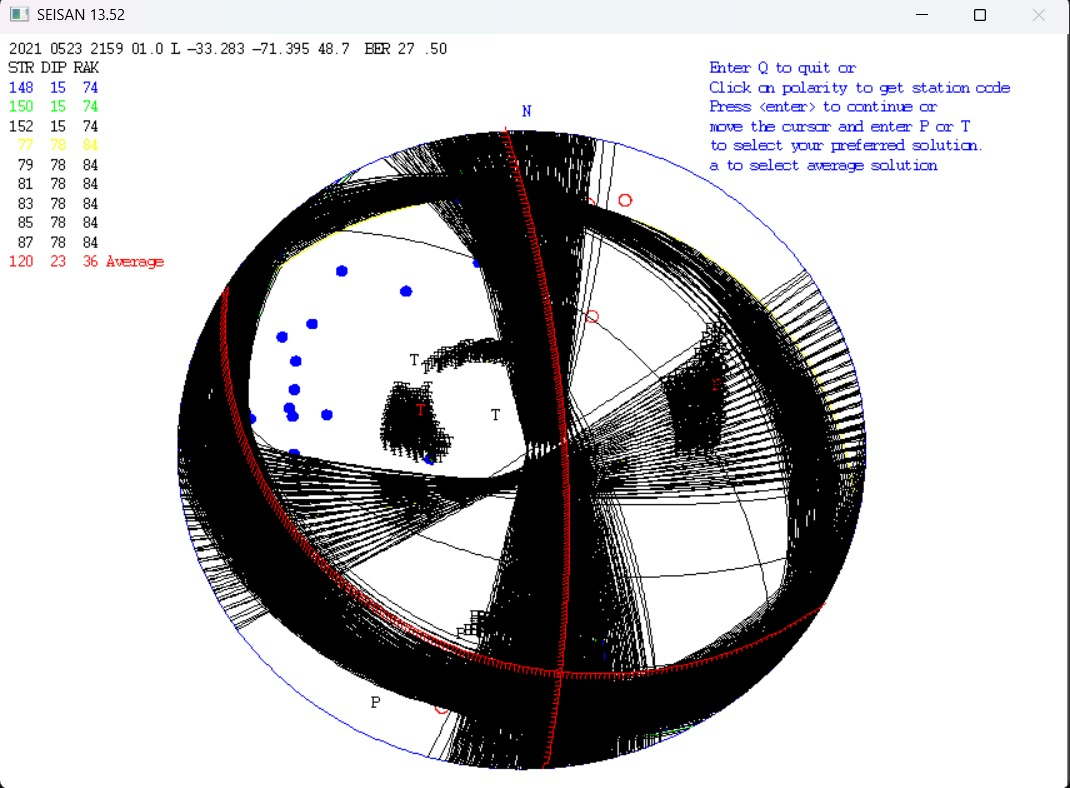
\includegraphics[width=\textwidth]{Figures/mecanismo_FOCMEC_20210523}
        \caption{Conjunto de soluciones de mecanismo focal calculadas mediante \texttt{FOCMEC} para el evento del 23 de mayo de 2021. La solución promedio indicada por el programa presenta \textit{strike} $120^\circ$, \textit{dip} $23^\circ$ y \textit{rake} $36^\circ$.}
        \label{fig:focmec-evento-20210523}
    \end{subfigure}
    \hfill
    \begin{subfigure}[b]{0.49\textwidth}
        \centering
        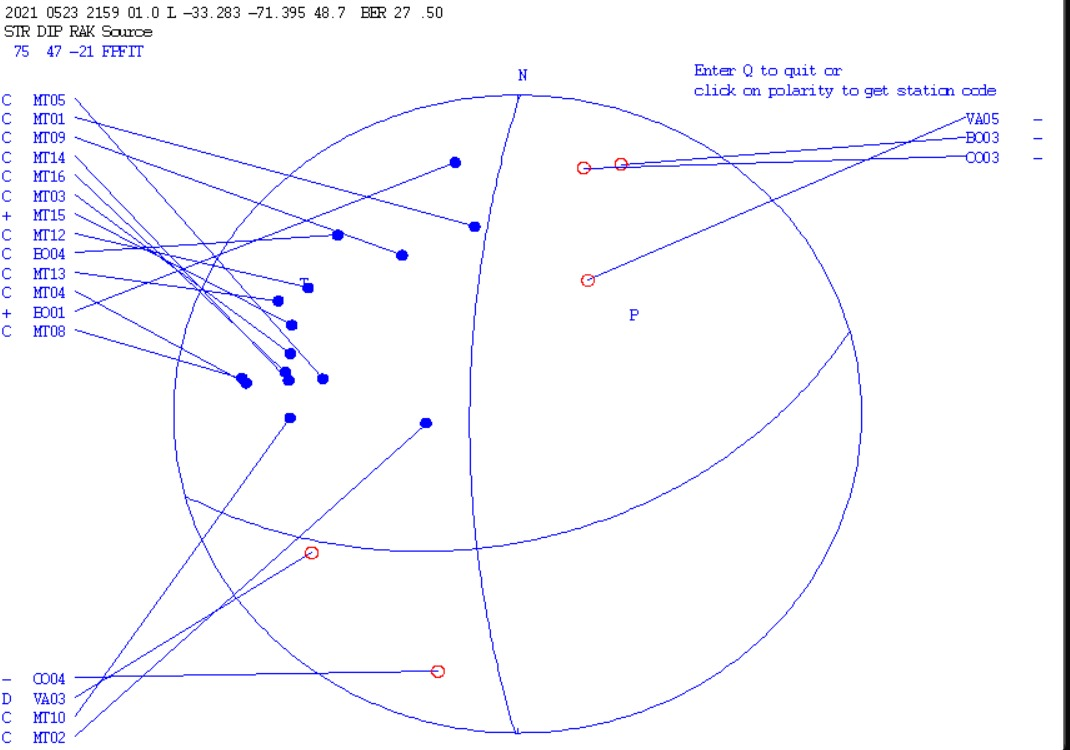
\includegraphics[width=\textwidth]{Figures/mecanismo_FPFIT_20210523}
        \caption{Solución de mecanismo focal calculada mediante \texttt{FPFIT} para el evento del 23 de mayo de 2021. El mecanismo presenta \textit{strike} $75^\circ$, \textit{dip} $47^\circ$ y \textit{rake} $-21^\circ$.}
        \label{fig:fpfit-evento-20210523}
    \end{subfigure}

    \caption{Soluciones de mecanismo focal obtenidas para el evento del 23 de mayo de 2021 mediante los programas \texttt{FOCMEC} y \texttt{FPFIT}.}
    \label{fig:mecanismos-evento-20210523}
\end{figure}

A partir de las polaridades de las primeras llegadas de ondas P seleccionadas para el evento del 23 de mayo de 2021, se calcularon mecanismos focales mediante los programas \texttt{FOCMEC} y \texttt{FPFIT}. La Figura~\ref{fig:mecanismos-evento-20210523} presenta las soluciones gráficas obtenidas mediante ambos procedimientos, representadas mediante diagramas de hemisferio inferior o ``pelotas de playa''. En estas representaciones, los símbolos rellenos corresponden a polaridades compresionales y los símbolos vacíos a polaridades dilatacionales, mientras que las curvas delimitan los planos nodales asociados a cada solución.

El cálculo realizado con \texttt{FOCMEC} entregó múltiples soluciones admisibles, debido a las combinaciones de \textit{strike}, \textit{dip} y \textit{rake} compatibles con las polaridades disponibles. La Figura~\ref{fig:mecanismos-evento-20210523}a muestra el conjunto de soluciones exploradas por el programa, incluyendo la solución promedio resaltada. Para esta solución promedio, \texttt{FOCMEC} reportó un \textit{strike} de $120^\circ$, un \textit{dip} de $23^\circ$ y un \textit{rake} de $36^\circ$. La visualización también incluye los ejes principales asociados al mecanismo y la distribución de las polaridades empleadas.

Por su parte, \texttt{FPFIT} entregó una solución con \textit{strike} de $75^\circ$, \textit{dip} de $47^\circ$ y \textit{rake} de $-21^\circ$, como se muestra en la Figura~\ref{fig:mecanismos-evento-20210523}b. La salida numérica del programa reportó un valor de ajuste (\textit{fit}) de $0{,}000$ y errores estimados de $14^\circ$ para el \textit{strike}, $25^\circ$ para el \textit{dip} y $18^\circ$ para el \textit{rake}. Estos valores corresponden a las incertidumbres angulares estimadas para los parámetros geométricos de la solución obtenida mediante el ajuste de las polaridades.

\subsection{Evento del 10 de diciembre de 2022}

Para el segundo evento seleccionado, correspondiente al archivo \texttt{event20221210T072548}, se repitió el procedimiento de procesamiento aplicado al evento anterior. En particular, se revisaron las formas de onda disponibles, se identificaron y marcaron manualmente los arribos de las fases P y S en las estaciones con señales utilizables y se registraron las polaridades de las primeras llegadas P cuando fue posible reconocerlas. Posteriormente, los tiempos seleccionados fueron utilizados por SEISAN para calcular una solución de localización mediante el modelo de velocidades configurado.

Este evento presentó una mayor dificultad durante el proceso de picado y ajuste de las fases, principalmente debido a que las diferencias entre los tiempos observados y los tiempos teóricos fueron más marcadas en varias estaciones. Como resultado, la mejor solución obtenida alcanzó un valor de \textit{RMS} de aproximadamente $0{,}8$~s, superior al criterio de $0{,}5$~s definido inicialmente para la actividad. Aun así, esta solución se conservó como el mejor resultado alcanzado durante el procesamiento, dado que representa el ajuste más consistente obtenido a partir de los picks manuales seleccionados.

\begin{figure}[h]
    \centering
    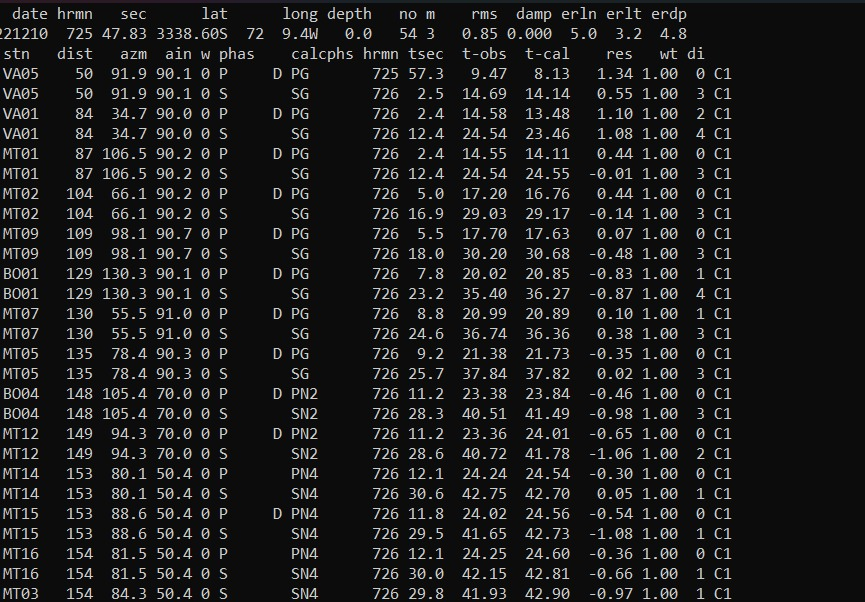
\includegraphics[width=0.80\textwidth]{Figures/RMS_2}
    \caption{Salida de SEISAN para la localización del evento del 10 de diciembre de 2022. La figura muestra los parámetros de la solución hipocentral, las fases P y S utilizadas, los tiempos de viaje observados y calculados, y los residuos temporales asociados a cada observación. La mejor solución obtenida presentó un \textit{RMS} aproximado de $0{,}8$~s, calculado a partir de $54$ observaciones.}
    \label{fig:residuos-localizacion-20221210}
\end{figure}

La Figura~\ref{fig:residuos-localizacion-20221210} presenta la salida de SEISAN asociada a esta localización. En ella se muestran los parámetros de la solución calculada, las observaciones de fases P y S incorporadas en el ajuste, los tiempos de viaje observados y teóricos, así como los residuos temporales para cada estación. La cabecera indica una localización aproximada de $33{,}39^\circ$S y $72{,}16^\circ$W, con una profundidad de $0{,}0$~km, obtenida a partir de $54$ observaciones. El valor de \textit{RMS} mostrado por la salida es cercano a $0{,}85$~s, el cual se reporta como aproximadamente $0{,}8$~s para efectos de síntesis de los resultados.

\subsubsection{Soluciones de mecanismo focal}

\begin{figure}[h]
    \centering

    \begin{subfigure}[b]{0.49\textwidth}
        \centering
        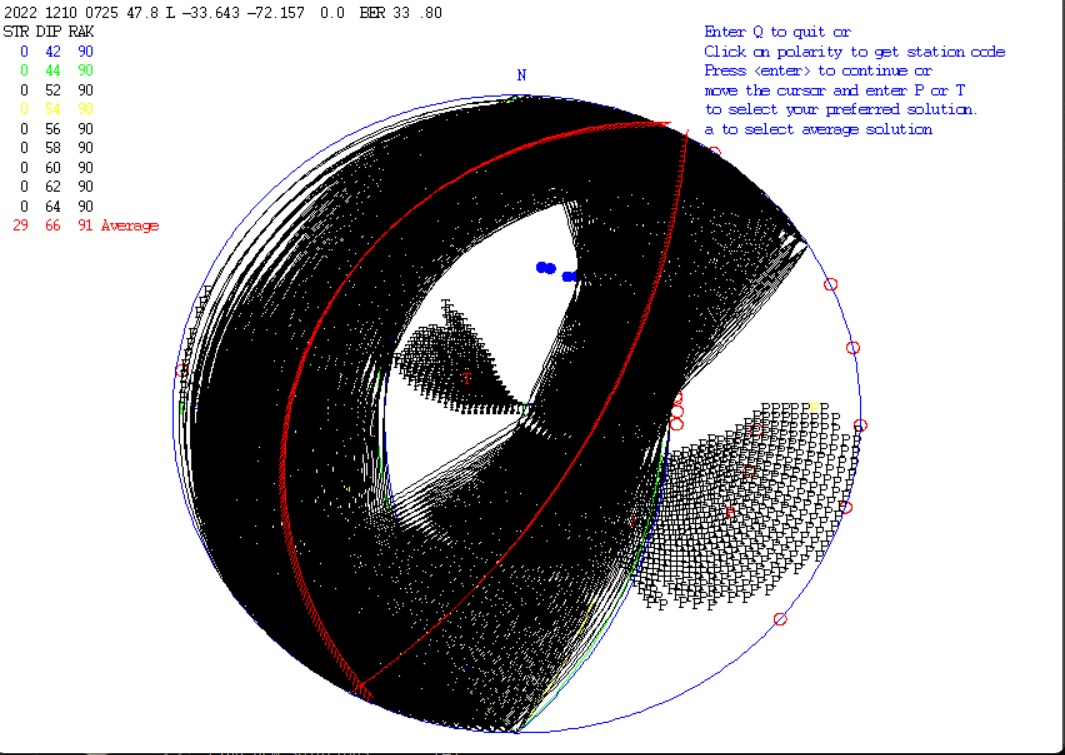
\includegraphics[width=\textwidth]{Figures/mecanismo_FOCMEC_20221210}
        \caption{Conjunto de soluciones de mecanismo focal calculadas con \texttt{FOCMEC} para el evento del 10 de diciembre de 2022. La solución promedio reportada presenta \textit{strike} $29^\circ$, \textit{dip} $66^\circ$ y \textit{rake} $91^\circ$.}
        \label{fig:focmec-evento-20221210}
    \end{subfigure}
    \hfill
    \begin{subfigure}[b]{0.49\textwidth}
        \centering
        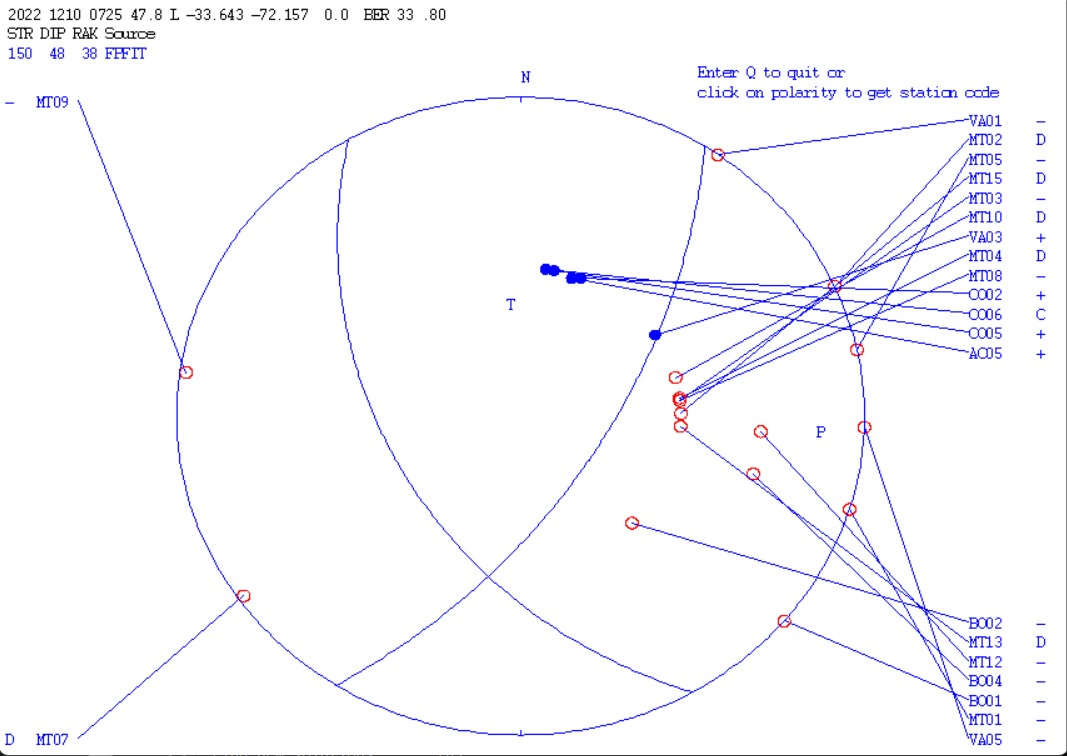
\includegraphics[width=\textwidth]{Figures/mecanismo_FPFIT_20221210}
        \caption{Solución de mecanismo focal calculada con \texttt{FPFIT} para el evento del 10 de diciembre de 2022. El mecanismo obtenido presenta \textit{strike} $150^\circ$, \textit{dip} $48^\circ$ y \textit{rake} $38^\circ$.}
        \label{fig:fpfit-evento-20221210}
    \end{subfigure}

    \caption{Soluciones de mecanismo focal obtenidas para el evento del 10 de diciembre de 2022 mediante los programas \texttt{FOCMEC} y \texttt{FPFIT}.}
    \label{fig:mecanismos-evento-20221210}
\end{figure}

Para el evento del 10 de diciembre de 2022 se calcularon mecanismos focales a partir de las polaridades de las primeras llegadas de ondas P seleccionadas durante el procesamiento de las formas de onda. Las soluciones fueron estimadas mediante los programas \texttt{FOCMEC} y \texttt{FPFIT}. La Figura~\ref{fig:mecanismos-evento-20221210} presenta los diagramas obtenidos con ambos programas. En estas representaciones, los símbolos rellenos corresponden a polaridades compresionales y los símbolos vacíos corresponden a polaridades dilatacionales; las curvas representan los planos nodales de las soluciones calculadas.

El resultado de \texttt{FOCMEC}, mostrado en la Figura~\ref{fig:focmec-evento-20221210}, contiene un conjunto de soluciones compatibles con las polaridades disponibles. La solución promedio reportada por el programa presenta un \textit{strike} de $29^\circ$, un \textit{dip} de $66^\circ$ y un \textit{rake} de $91^\circ$. La figura muestra además la distribución de las polaridades utilizadas y los ejes principales asociados a la solución promedio, así como la existencia de varias soluciones admisibles dentro del espacio de búsqueda.

Por su parte, \texttt{FPFIT} entregó una solución con \textit{strike} de $150^\circ$, \textit{dip} de $48^\circ$ y \textit{rake} de $38^\circ$, representada en la Figura~\ref{fig:fpfit-evento-20221210}. La salida numérica de \texttt{FPFIT} reportó un valor de ajuste (\textit{fit}) de $0{,}000$, junto con errores estimados de $1^\circ$ para el \textit{strike}, $2^\circ$ para el \textit{dip} y $12^\circ$ para el \textit{rake}. Estos valores resumen los parámetros geométricos y las incertidumbres angulares obtenidas para la solución calculada por el programa; la captura de esta salida se conserva como registro numérico del procesamiento, pero no se incorpora como figura en el informe.


\newpage

\section{Discusión}

\subsection{Clasificación sismotectónica de los eventos a partir de la localización y los mecanismos focales}

\subsubsection{Evento del 23 de mayo de 2021}

La solución obtenida mediante SEISAN para el evento del 23 de mayo de 2021 ubica el hipocentro aproximadamente en $33{,}16^\circ$S y $71{,}24^\circ$W, a una profundidad de $48{,}4$~km. Esta posición se encuentra frente a la costa de Chile central, en el margen oceánico próximo a la región de Valparaíso, y a una profundidad compatible con la zona de contacto entre la placa de Nazca y la placa Sudamericana. La localización se obtuvo utilizando 51 observaciones de fases P y S y presenta un \textit{RMS} de $0{,}48$~s, valor inferior al criterio de $0{,}5$~s definido para la actividad. Por tanto, dentro de las limitaciones del modelo de velocidades y de la distribución de estaciones, esta es la solución con mejor ajuste temporal de los dos eventos analizados.

La combinación de la ubicación en planta, la profundidad hipocentral y el contexto regional permite clasificar este evento de manera preliminar como un sismo asociado a la subducción, probablemente de tipo interplaca o próximo al límite interplaca. La posición al oeste de la línea de costa y la profundidad cercana a 50~km son consistentes con la geometría esperada de la placa de Nazca al introducirse bajo la placa Sudamericana en el segmento central de Chile. En esta zona, la sismicidad se concentra principalmente en el contacto entre placas y en sectores próximos a la interfaz, donde la convergencia relativa produce acumulación y liberación de esfuerzos.

No obstante, la clasificación debe considerarse con prudencia, debido a que la profundidad de $48{,}4$~km se encuentra en una zona de transición entre la sismicidad interplaca más superficial y la sismicidad que puede ocurrir dentro de la placa subducida. En consecuencia, la localización por sí sola no permite descartar de manera absoluta una fuente intraplaca oceánica cercana al plano de subducción. La interpretación preferida como evento interplaca se sustenta principalmente en que el hipocentro se sitúa mar adentro, aproximadamente en el rango de profundidades esperado para la interfaz en esta latitud, y en que los mecanismos focales calculados presentan componentes compatibles con un régimen tectónico compresivo asociado a la convergencia.

Los resultados de mecanismo focal aportan información adicional, pero también muestran dispersión entre métodos. \texttt{FOCMEC} entregó un conjunto de soluciones admisibles y una solución promedio de \textit{strike} $120^\circ$, \textit{dip} $23^\circ$ y \textit{rake} $36^\circ$. Por su parte, \texttt{FPFIT} estimó una solución de \textit{strike} $75^\circ$, \textit{dip} $47^\circ$ y \textit{rake} $-21^\circ$, con incertidumbres de $14^\circ$, $25^\circ$ y $18^\circ$ para \textit{strike}, \textit{dip} y \textit{rake}, respectivamente. Estas dos soluciones no son idénticas y no permiten asignar un mecanismo puro de manera inequívoca; sin embargo, ambas incluyen una componente de deslizamiento oblicuo y son compatibles con un campo de esfuerzos complejo en el margen de subducción.

El valor positivo del \textit{rake} promedio obtenido con \texttt{FOCMEC} indica una componente inversa, mientras que el valor ligeramente negativo obtenido con \texttt{FPFIT} sugiere una componente oblicua con participación normal o de rumbo, dependiendo del plano nodal considerado. Esta diferencia puede relacionarse con la distribución azimutal no homogénea de las estaciones, la cantidad limitada de polaridades utilizables, la cercanía de algunas observaciones a los planos nodales y las incertidumbres en la localización. En consecuencia, los mecanismos focales permiten reconocer que el evento no corresponde a una ruptura cortical simple, sino a una fuente situada en una región tectónica de subducción, con un mecanismo focal que requiere ser interpretada en conjunto con la geometría regional de la placa y contrastada con información de otras fuentes.

En síntesis, el evento del 23 de mayo de 2021 se interpreta preferentemente como un sismo de subducción de profundidad intermedia superficial, probablemente asociado a la interfaz Nazca--Sudamérica o a un sector inmediatamente adyacente dentro de la placa de Nazca subducida. La solución hipocentral posee un ajuste temporal satisfactorio, y la ubicación mar adentro junto con la profundidad cercana a 50~km constituye la evidencia principal de esta clasificación. La variabilidad entre las soluciones de \texttt{FOCMEC} y \texttt{FPFIT} indica, sin embargo, que la geometría exacta de la falla y el tipo de deslizamiento deben considerarse con un nivel moderado de incertidumbre.

\subsubsection{Evento del 10 de diciembre de 2022}

Para el evento del 10 de diciembre de 2022, la solución obtenida mediante SEISAN se localiza aproximadamente en $33{,}39^\circ$S y $72{,}16^\circ$W, con una profundidad calculada de $0{,}0$~km. Esta localización se sitúa mar adentro, al oeste de la costa de Chile central, y por lo tanto dentro del dominio oceánico o del margen externo de subducción. Sin embargo, la solución debe interpretarse con especial cautela, ya que el mejor ajuste alcanzado presentó un \textit{RMS} cercano a $0{,}85$~s, superior al criterio de $0{,}5$~s propuesto para la actividad. Además, una profundidad fijada o ajustada a $0{,}0$~km puede indicar que la profundidad no quedó adecuadamente restringida por los datos disponibles y no debe asumirse automáticamente como la profundidad física exacta del hipocentro.

La posición en planta, aproximadamente un grado más al oeste que la solución del evento de 2021, permite proponer que este sismo se produjo en el ambiente oceánico previo a la subducción. Si la profundidad superficial obtenida fuese representativa de la fuente real, el evento podría clasificarse como sismicidad intraplaca oceánica superficial o \emph{outer-rise}, asociada a la deformación de la placa de Nazca antes de ingresar en la fosa. Este tipo de eventos se localiza mar adentro y puede estar vinculado con esfuerzos de flexión de la placa oceánica.

Los mecanismos focales calculados para este evento también muestran diferencias importantes entre ambos programas. La solución promedio de \texttt{FOCMEC} presenta \textit{strike} $29^\circ$, \textit{dip} $66^\circ$ y \textit{rake} $91^\circ$. Un \textit{rake} cercano a $90^\circ$ corresponde a un mecanismo predominantemente inverso, es decir, a una componente compresiva significativa. En contraste, \texttt{FPFIT} entregó una solución de \textit{strike} $150^\circ$, \textit{dip} $48^\circ$ y \textit{rake} $38^\circ$, correspondiente a un mecanismo oblicuo con una componente inversa. Aunque ambas soluciones no coinciden en la orientación del plano nodal, las dos sugieren una componente de compresión o de deslizamiento inverso.

La presencia de mecanismos con componente inversa no descarta completamente una fuente oceánica, pues la flexión de la placa de Nazca puede generar distintos regímenes de esfuerzo en profundidad. No obstante, si el evento estuviera realmente asociado al \emph{outer-rise} más superficial, sería común esperar mecanismos con una mayor componente normal, vinculados a extensión por curvatura de la placa. Por esta razón, la combinación entre una localización superficial poco restringida y mecanismos focales que sugieren compresión no permite asignar de manera inequívoca el evento a una categoría sismotectónica única.

Una interpretación alternativa es que la localización obtenida no represente de forma precisa la profundidad real del evento y que el sismo haya ocurrido a mayor profundidad, posiblemente en la interfaz de subducción o dentro de la placa oceánica subducida. Esta posibilidad es consistente con la discrepancia entre los tiempos observados y calculados, el valor de \textit{RMS} superior a $0{,}8$~s y la diferencia entre los mecanismos focales obtenidos con \texttt{FOCMEC} y \texttt{FPFIT}. Sin una solución hipocentral más estable o una comparación directa con la localización oficial de una agencia sismológica, no es posible decidir con certeza entre una fuente superficial oceánica, una fuente interplaca o una fuente intraplaca.

\newpage

\subsection{Diferencias entre los tiempos de llegada observados y teóricos}

Los tiempos de llegada observados para las fases P y S no coinciden necesariamente con los tiempos teóricos calculados por SEISAN, porque ambos provienen de procesos distintos. El tiempo observado se obtiene mediante el picado manual sobre la forma de onda registrada en cada estación y representa la mejor estimación del instante en que comienza físicamente la llegada de una fase. En contraste, el tiempo teórico es una predicción calculada por el programa a partir de una localización tentativa del sismo, las coordenadas de la estación y un modelo de velocidades sísmicas. Por ello, la diferencia entre ambos tiempos, denominada residuo, es una medida directa de la discrepancia entre la propagación real de las ondas y la propagación prevista por el modelo.

Para calcular un tiempo teórico, SEISAN parte de una hipótesis inicial de hipocentro, definida por la latitud, longitud, profundidad y tiempo de origen. A continuación, utiliza las coordenadas de cada estación incluidas en el archivo \texttt{STATION0.HYP} para determinar la distancia y la geometría entre la fuente y el receptor. Con esta información, el programa calcula el trayecto de rayos y el tiempo de viaje esperado para las ondas P y S de acuerdo con las velocidades asignadas a las capas del modelo. Posteriormente, compara el tiempo calculado con el tiempo de llegada observado. A partir del conjunto de residuos de todas las estaciones, SEISAN ajusta iterativamente los parámetros hipocentrales hasta minimizar el error global, expresado mediante el valor de \textit{RMS}.

El archivo \texttt{STATION0.HYP} utilizado en esta actividad contiene las coordenadas de las estaciones de las redes C1 y CX, además de un modelo de velocidad dependiente de la profundidad. El modelo asigna velocidades de onda P crecientes desde aproximadamente $4{,}08$~km/s en superficie hasta valores cercanos a $8{,}23$~km/s a 75~km de profundidad. Por ejemplo, el modelo considera velocidades P de $4{,}57$~km/s a 1~km, $5{,}72$~km/s a 7~km, $6{,}64$~km/s a 19~km, $6{,}99$~km/s a 33~km, $7{,}61$~km/s a 45~km y $8{,}23$~km/s a 75~km de profundidad. Asimismo, el archivo define una relación global aproximada

\[
\frac{V_P}{V_S}=1{,}74,
\]

a partir de la cual se estima la velocidad de las ondas S. De este modo, el modelo representa la estructura terrestre mediante un conjunto de capas horizontales, dentro de las cuales la velocidad se considera constante o cambia únicamente en función de la profundidad.

Esta representación es útil para localizar eventos de manera operacional, pero implica simplificaciones importantes. El modelo no reproduce en detalle las variaciones laterales de velocidad, la topografía del Moho, la geometría tridimensional de la placa de Nazca, el contacto irregular entre las placas, los cambios de composición de la corteza continental y oceánica, ni las heterogeneidades locales asociadas a fracturas, volcanismo, cuencas sedimentarias o variaciones térmicas. En una zona de subducción como Chile central, las ondas pueden atravesar materiales con propiedades muy diferentes: corteza oceánica, sedimentos, corteza continental y la placa oceánica subducida. Cada una de estas unidades posee velocidades y estructuras distintas, por lo que los trayectos reales de las ondas P y S pueden desviarse respecto de los rayos simplificados considerados por un modelo unidimensional.

La predicción de los arribos también se complica porque la geometría de la fuente no es conocida antes de realizar la localización. La profundidad, el tiempo de origen y la posición horizontal del hipocentro afectan los tiempos de viaje de manera simultánea. Por ejemplo, un cambio en la profundidad puede modificar los tiempos calculados de P y S para todas las estaciones, pero con efectos distintos según la distancia epicentral y la dirección de cada receptor. De forma similar, una estación ubicada sobre roca competente puede registrar fases con una apariencia más definida que otra instalada sobre depósitos superficiales, donde la señal puede estar afectada por amplificación, dispersión o ruido local. Estas condiciones dificultan establecer el instante exacto del primer arribo, especialmente para fases emergentes.

Las diferencias entre los dos eventos procesados ilustran este comportamiento. Para el evento del 23 de mayo de 2021 se obtuvo un \textit{RMS} de $0{,}48$~s, lo que indica una concordancia global relativamente buena entre los tiempos seleccionados y los tiempos calculados por el modelo. Sin embargo, incluso en esta solución se observaron residuos individuales positivos y negativos, incluyendo algunos cercanos a $-1{,}00$~s y otros de hasta aproximadamente $0{,}88$~s. Para el evento del 10 de diciembre de 2022, el mejor ajuste alcanzó un \textit{RMS} cercano a $0{,}85$~s, con residuos individuales que llegaron aproximadamente a $1{,}34$~s y $-1{,}08$~s. Este contraste muestra que la capacidad de ajuste depende de la calidad de las fases identificadas, de la cobertura geométrica de las estaciones y de qué tan representativo resulte el modelo de velocidades para la trayectoria real de las ondas en cada evento.

Por lo tanto, los picks observados no deben desplazarse artificialmente hasta coincidir con los tiempos teóricos únicamente para disminuir el \textit{RMS}. El pick debe mantenerse en el punto donde se identifica el inicio físico más confiable de la fase en la señal. Forzar su coincidencia con la predicción del modelo eliminaría los residuos de manera artificial, sesgaría la localización y ocultaría las limitaciones del modelo de velocidades. El objetivo del procedimiento de localización es encontrar la solución hipocentral que explique de la mejor manera posible el conjunto de observaciones reales, no modificar las observaciones para que se adapten exactamente a un modelo simplificado.

En consecuencia, los residuos entre tiempos observados y teóricos son esperables y contienen información relevante sobre la calidad del ajuste. Un valor de \textit{RMS} bajo sugiere una buena consistencia global entre los picks, la localización y el modelo de velocidades, mientras que residuos elevados o patrones sistemáticos de residuos positivos o negativos pueden indicar incertidumbres en los arribos seleccionados, limitaciones de la geometría de la red o la necesidad de emplear un modelo de velocidades más representativo de la estructura tridimensional de la zona de subducción.


\subsection{¿Es posible constreñir los mecanismos focales con las observaciones existentes? ¿Hay diferencias entre las soluciones que entregan FPFIT y FOCMEC?}

Los mecanismos focales pueden constreñirse de manera parcial con las observaciones disponibles, pero el nivel de restricción no es suficiente para considerar las soluciones obtenidas como únicas o completamente definidas. Esto se debe a que la calidad de esta estimación depende no sólo de la cantidad de polaridades disponibles, sino principalmente de su cobertura azimutal y de la confiabilidad de cada observación.

En los eventos analizados, las figuras de \texttt{FOCMEC} muestran que las estaciones no presentan una distribución azimutal completamente homogénea. En ambos casos, varias observaciones se concentran hacia sectores específicos del hemisferio focal, mientras que otros cuadrantes presentan una cobertura reducida o ausente. Esta geometría limita la capacidad para discriminar de forma única entre los dos planos nodales y para determinar con precisión la orientación real del plano de falla. Además, algunas polaridades se ubican próximas a los límites entre cuadrantes de compresión y dilatación, donde el aporte a la determinación de la magnitud focal es significativamente menor.

El resultado de \texttt{FOCMEC} para el evento del 23 de mayo de 2021 evidencia esta limitación de manera directa. El programa encontró múltiples soluciones admisibles y calculó una solución promedio de rumbo $120^\circ$, \textit{dip} $23^\circ$ y \textit{rake} $36^\circ$. La existencia de numerosas soluciones compatibles indica que las polaridades disponibles permiten restringir un rango de mecanismos posibles, pero no seleccionar una única solución con total seguridad. El resultado de \texttt{FPFIT}, con \textit{strike} $75^\circ$, \textit{dip} $47^\circ$ y \textit{rake} $-21^\circ$, difiere de la solución promedio de \texttt{FOCMEC}. Aunque ambas soluciones se ajustan al conjunto de polaridades bajo sus respectivos criterios, la diferencia entre ellas muestra que la orientación exacta de los planos nodales no está fuertemente constreñida. Las incertidumbres entregadas por \texttt{FPFIT}, de $14^\circ$ en \textit{strike}, $25^\circ$ en \textit{dip} y $18^\circ$ en \textit{rake}, refuerzan esta conclusión.

Para el evento del 10 de diciembre de 2022, la restricción es todavía más limitada debido a que la localización alcanzó un \textit{RMS} de aproximadamente $0{,}85$~s y una profundidad de $0{,}0$~km. La incertidumbre en la profundidad afecta directamente el cálculo de los ángulos de salida de los rayos desde el hipocentro hacia las estaciones, y dichos ángulos son esenciales para proyectar correctamente las polaridades sobre el hemisferio focal. En este caso, \texttt{FOCMEC} también generó un conjunto amplio de soluciones admisibles, con una solución promedio de rumbo $29^\circ$, \textit{dip} $66^\circ$ y \textit{rake} $91^\circ$. \texttt{FPFIT}, en cambio, entregó rumbo $150^\circ$, \textit{dip} $48^\circ$ y \textit{rake} $38^\circ$. La diferencia entre ambos resultados es considerable y evidencia que, aunque las polaridades imponen ciertas restricciones sobre el tipo general de deformación, no permiten definir una geometría focal única.

En consecuencia, las observaciones existentes permiten establecer mecanismos focales preliminares y reconocer tendencias generales en el tipo de deformación, como la presencia de componentes inversas u oblicuas en las soluciones obtenidas. Sin embargo, no permiten definir sin ambigüedad el plano de falla, ni asignar una solución única de \textit{strike}, \textit{dip} y \textit{rake} para ninguno de los dos eventos.


\subsection{Comparación con soluciones de agencias sismológicas}

La comparación entre las soluciones obtenidas mediante SEISAN y los catálogos de agencias sismológicas debe considerar que las localizaciones elaboradas en este trabajo se basan en un subconjunto de registros, en picks manuales de fases P y S, y en un modelo de velocidades unidimensional incluido en el archivo \texttt{STATION0.HYP}. En cambio, instituciones como el Centro Sismológico Nacional de Chile (CSN) y el United States Geological Survey (USGS) procesan los eventos mediante redes más extensas, catálogos operacionales, procedimientos de control de calidad y modelos de localización que pueden diferir del utilizado en esta actividad~\cite{CSNEventDatabase,USGSEarthquakeCatalog}.

\subsubsection{Evento del 23 de mayo de 2021}

La localización obtenida en SEISAN para el evento del 23 de mayo de 2021 fue de aproximadamente $33{,}16^\circ$S, $71{,}24^\circ$W y $48{,}4$~km de profundidad, con un \textit{RMS} de $0{,}48$~s. La solución de referencia reportada para el mismo instante por el USGS corresponde al evento \texttt{us7000e5lp}, ocurrido el 23 de mayo de 2021 a las 21:58:59 UTC, de magnitud 4,6, localizado aproximadamente a $33{,}2875^\circ$S y $71{,}396^\circ$W, con una profundidad de 53,85~km y una referencia espacial cercana a Quilpué~\cite{USGS2021Quilpue}.

Por tanto, la solución obtenida en este trabajo presenta una buena concordancia general con la referencia del USGS. La diferencia horizontal entre ambas soluciones es del orden de decenas de kilómetros, mientras que la diferencia de profundidad es cercana a 5~km. Estas discrepancias son razonables considerando que el cálculo realizado en SEISAN utilizó 51 observaciones y un modelo de velocidades simplificado, mientras que la solución de la USGS puede incorporar información de una red más amplia, procedimientos automáticos y revisiones posteriores.

La cercanía entre ambas profundidades es particularmente relevante, porque ambas sitúan el evento en torno a 50~km de profundidad, es decir, bajo la zona costera y dentro del dominio de subducción. En consecuencia, tanto la localización propia como la solución de referencia respaldan la interpretación de un evento relacionado con el sistema de subducción Nazca--Sudamérica, más que con una fuente cortical superficial. La pequeña diferencia en latitud, longitud y profundidad puede explicarse por la cobertura efectiva de estaciones empleada, la sensibilidad de la profundidad a los tiempos de llegada, los residuos de cada fase y las limitaciones de representar una estructura tectónica tridimensional con un modelo de velocidades dependiente solamente de la profundidad.

En cuanto al mecanismo focal, los resultados propios obtenidos con \texttt{FOCMEC} y \texttt{FPFIT} deben interpretarse como soluciones preliminares. La solución de \texttt{FOCMEC} presentó un conjunto de mecanismos admisibles, con una solución promedio de rumbo $120^\circ$, manteo $23^\circ$ y \textit{rake} $36^\circ$; \texttt{FPFIT} entregó rumbo $75^\circ$, manteo $47^\circ$ y \textit{rake} $-21^\circ$. La diferencia entre ambos métodos indica que las polaridades disponibles no constreñen de manera única la geometría de los planos nodales. Desafortunadamente, no existe mecanismo focal disponible por el USGS, por lo que el mecanismo focal derivado en este ejercicio es el único de comparación y debe utilizarse principalmente para reconocer una componente de deformación oblicua en un contexto de subducción y no como una solución focal definitiva.

\subsubsection{Evento del 10 de diciembre de 2022}

Para el evento del 10 de diciembre de 2022, la comparación con la solución publicada por el USGS confirma que la localización obtenida mediante SEISAN presenta diferencias importantes, particularmente en profundidad. El USGS reporta para el evento \texttt{us6000j8d7} una magnitud de momento de Mw~5{,}4 $\pm 0{,}1$, con tiempo de origen el 10 de diciembre de 2022 a las 07:25:48.073 UTC, una localización de $33{,}646^\circ$S y $72{,}079^\circ$W, con una incertidumbre horizontal de $\pm 4{,}1$~km, y una profundidad de $21{,}7 \pm 3{,}6$~km.\cite{USGS2022OffshoreChile}

La solución calculada en este trabajo mediante SEISAN fue de aproximadamente $33{,}39^\circ$S, $72{,}16^\circ$W y una profundidad de $0{,}0$~km, con un \textit{RMS} de $0{,}85$~s. En planta, ambas soluciones se ubican mar adentro frente a la costa central de Chile y muestran una concordancia regional aceptable. Sin embargo, la diferencia en latitud es cercana a $0{,}26^\circ$, equivalente aproximadamente a 29~km en dirección norte--sur, mientras que la diferencia longitudinal es cercana a $0{,}08^\circ$, del orden de 7--8~km a esta latitud. La discrepancia más relevante corresponde a la profundidad: el USGS ubica el hipocentro a aproximadamente 22~km, mientras que la solución obtenida con SEISAN alcanza el límite superficial de $0{,}0$~km.

Esta diferencia indica que, para el conjunto de picks y el modelo de velocidades utilizado, la profundidad no quedó adecuadamente constreñida. El valor superficial calculado por SEISAN no debe interpretarse como una demostración de que el evento ocurrió literalmente en superficie; por el contrario, el \textit{RMS} de $0{,}85$~s, superior al criterio de $0{,}5$~s definido para la actividad, y la presencia de residuos individuales considerables evidencian una capacidad limitada para reproducir simultáneamente los tiempos de llegada observados. La solución del USGS, con una profundidad intermedia de $21{,}7$~km, es más consistente con un evento ocurrido dentro del sistema de subducción frente a la costa de Chile central~\cite{USGS2022OffshoreChile}.

La comparación de los mecanismos focales también muestra coincidencias parciales y diferencias en la geometría de los planos nodales. El mecanismo de referencia publicado por el USGS, mostrado en la Figura~\ref{fig:usgs-mecanismo-evento-20221210}, presenta dos planos nodales: el plano NP1 tiene \textit{strike} $186^\circ$, \textit{dip} $66^\circ$ y \textit{rake} $88^\circ$, mientras que el plano NP2 tiene \textit{strike} $12^\circ$, \textit{dip} $24^\circ$ y \textit{rake} $95^\circ$~\cite{USGS2022OffshoreChile}. Ambos planos presentan un \textit{rake} cercano a $+90^\circ$, lo que corresponde a un mecanismo predominantemente inverso, compatible con un régimen compresivo.

\begin{figure}[htbp]
    \centering
    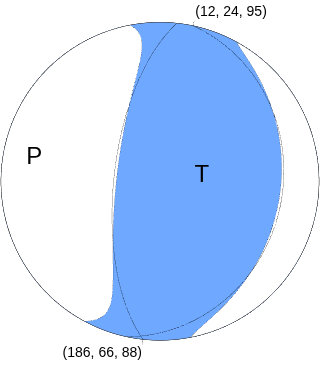
\includegraphics[width=0.35\textwidth]{Figures/Mecanismosegundo}
    \caption{Mecanismo focal publicado por el USGS para el evento \texttt{us6000j8d7}, ocurrido el 10 de diciembre de 2022. Los planos nodales reportados son: NP1, rumbo $186^\circ$, manteo $66^\circ$ y \textit{rake} $88^\circ$; y NP2, rumbo $12^\circ$, manteo $24^\circ$ y \textit{rake} $95^\circ$. La solución corresponde a un mecanismo predominantemente inverso. \cite{USGS2022OffshoreChile}}
    \label{fig:usgs-mecanismo-evento-20221210}
\end{figure}

La solución promedio obtenida con \texttt{FOCMEC} presenta \textit{strike} $29^\circ$, \textit{dip} $66^\circ$ y \textit{rake} $91^\circ$. Esta solución conserva una coincidencia importante con el mecanismo del USGS: ambos presentan un \textit{dip} alto, cercano a $66^\circ$, y un \textit{rake}$\,$ cercano a $+90^\circ$, lo que indica una componente inversa dominante. Aunque el \textit{strike} de la solución de \texttt{FOCMEC} no coincide exactamente con el \textit{strike} de NP1, es relativamente próximo al \textit{strike} de NP2, considerando la ambigüedad inherente entre los dos planos nodales y las limitaciones de cobertura azimutal. Por lo tanto, \texttt{FOCMEC} reproduce de manera razonable el carácter inverso del mecanismo reportado por el USGS.

La solución obtenida con \texttt{FPFIT}, de \textit{strike} $150^\circ$, \textit{dip} $48^\circ$ y \textit{rake} $38^\circ$, presenta una concordancia menor con la solución de la agencia. Aunque mantiene una componente inversa positiva, su \textit{rake} es claramente inferior a los valores de $88^\circ$ y $95^\circ$ reportados por el USGS, lo que implica una contribución oblicua más importante. Además, el \textit{dip} de $48^\circ$ es menor que el de NP1 y mayor que el de NP2. Esta diferencia es coherente con la existencia de una cobertura de polaridades incompleta y con la incertidumbre de la localización propia, especialmente de la profundidad.

En síntesis, el análisis comparativo muestra que la localización propia y la solución del USGS coinciden en ubicar el evento mar adentro, frente al margen central de Chile, no obstante, difieren de forma relevante en la profundidad. La solución del USGS a 21,7~km, junto con su mecanismo inverso, permite interpretar el evento como un sismo asociado al régimen compresivo del margen de subducción de Chile. La solución de \texttt{FOCMEC} reproduce de manera consistente la componente inversa principal identificada por el USGS, mientras que la solución de \texttt{FPFIT} presenta una mayor componente oblicua. Estas diferencias son esperables debido a que el análisis de este trabajo se basa en un conjunto reducido de polaridades y en un modelo de velocidades simplificado, mientras que el USGS utiliza datos y procedimientos de localización e inversión de mayor alcance.

\section{Conclusiones}

La presente actividad permitió aplicar un flujo completo de procesamiento sismológico mediante SEISAN, desde la preparación de los archivos de trabajo y la visualización de formas de onda hasta el picado de fases P y S, la asignación de polaridades, la localización hipocentral y el cálculo de mecanismos focales mediante \texttt{FOCMEC} y \texttt{FPFIT}. El ejercicio evidenció que la calidad de los resultados depende de manera crítica de la correcta identificación de los arribos, de la relación señal--ruido de las trazas, de la distribución espacial de las estaciones y del modelo de velocidades utilizado.

Para el evento del 23 de mayo de 2021 se obtuvo una localización aproximada de $33{,}16^\circ$S, $71{,}24^\circ$W y $48{,}4$~km de profundidad, calculada a partir de 51 observaciones y con un \textit{RMS} de $0{,}48$~s. Este resultado cumple el criterio de ajuste definido para la actividad y muestra una concordancia razonable con la solución de referencia del USGS, que localiza el evento cerca de $33{,}2875^\circ$S, $71{,}396^\circ$W y a una profundidad de $53{,}85$~km.\cite{USGS2021Quilpue} La similitud entre ambas soluciones, particularmente en profundidad, permite asociar el evento con el sistema de subducción Nazca--Sudamérica bajo el margen central de Chile. Sin embargo, los mecanismos focales obtenidos mediante \texttt{FOCMEC} y \texttt{FPFIT} presentaron diferencias en los parámetros de rumbo, manteo y \textit{rake}, por lo que la geometría exacta de la falla debe considerarse como una solución preliminar con incertidumbre moderada.

El evento del 10 de diciembre de 2022 presentó una mayor dificultad de procesamiento. La solución obtenida mediante SEISAN se localizó aproximadamente en $33{,}39^\circ$S y $72{,}16^\circ$W, con profundidad de $0{,}0$~km y un \textit{RMS} de $0{,}85$~s. El valor elevado de \textit{RMS} y la profundidad superficial calculada indicaron que los datos disponibles no permitieron restringir adecuadamente la solución hipocentral, especialmente la componente vertical. La comparación con el USGS mostró que ambas soluciones ubican el evento mar adentro frente a Chile central, no obstante, el USGS reporta una localización de $33{,}646^\circ$S, $72{,}079^\circ$W y una profundidad de $21{,}7 \pm 3{,}6$~km.\cite{USGS2022OffshoreChile} Esta diferencia confirma que la profundidad de $0{,}0$~km obtenida en SEISAN debe interpretarse como una limitación del ajuste y no como la profundidad física definitiva del sismo.

La comparación de mecanismos focales para el evento de 2022 mostró que la solución promedio de \texttt{FOCMEC}, con rumbo $29^\circ$, manteo $66^\circ$ y \textit{rake} $91^\circ$, reproduce de manera razonable el carácter inverso del mecanismo publicado por el USGS. La solución de la USGS presenta los planos nodales NP1 ($186^\circ/66^\circ/88^\circ$) y NP2 ($12^\circ/24^\circ/95^\circ$), ambos compatibles con una componente inversa dominante~\cite{USGS2022OffshoreChile}. En contraste, la solución de \texttt{FPFIT}, con \textit{strike} $150^\circ$, \textit{dip} $48^\circ$ y \textit{rake} $38^\circ$, conserva una componente inversa, pero presenta una contribución oblicua más importante. Esta diferencia demuestra que las polaridades utilizadas permiten reconocer tendencias generales del régimen de esfuerzos, pero no siempre definir un único plano de falla o una solución focal completamente estable.

El análisis de los tiempos de llegada permitió comprobar que los tiempos observados y teóricos no deben coincidir de manera exacta. Los tiempos teóricos calculados por SEISAN dependen de una localización tentativa, de las coordenadas de las estaciones y de un modelo de velocidades simplificado. El archivo \texttt{STATION0.HYP} utilizado representa la estructura mediante velocidades de onda P que aumentan con la profundidad, desde aproximadamente $4{,}08$~km/s en superficie hasta $8{,}23$~km/s a 75~km de profundidad, y utiliza una relación aproximada $V_P/V_S=1{,}74$ para estimar la propagación de las ondas S. Esta aproximación no reproduce todas las heterogeneidades laterales ni la geometría tridimensional del sistema de subducción, por lo que los residuos entre los tiempos observados y calculados constituyen una respuesta esperable del proceso de localización.

En consecuencia, el valor de \textit{RMS} debe interpretarse como un indicador global de consistencia entre las observaciones, la solución hipocentral y el modelo de velocidades, pero no como el único criterio de calidad. Reducir artificialmente el \textit{RMS} desplazando los picks para forzar su coincidencia con los tiempos teóricos introduciría sesgos y eliminaría información relevante sobre las diferencias entre el modelo y la propagación real de las ondas. La selección manual debe conservar el instante más confiable del inicio físico de cada fase, especialmente cuando las señales son emergentes o presentan ruido.

Finalmente, las observaciones existentes permitieron constreñir de manera parcial los mecanismos focales de ambos eventos. La cantidad de polaridades disponibles fue suficiente para identificar soluciones admisibles y reconocer componentes inversas u oblicuas. Sin embargo, la distribución azimutal no homogénea de las estaciones, la presencia de polaridades cercanas a los planos nodales, la incertidumbre de las localizaciones y la existencia de múltiples soluciones compatibles limitaron la determinación de una solución focal única. Para mejorar la robustez de futuras estimaciones sería conveniente contar con mayor cobertura azimutal, más polaridades de primera llegada confiables, localizaciones con menor incertidumbre en profundidad, modelos de velocidad tridimensionales y, cuando estén disponibles, información complementaria de relaciones de amplitud, inversión de formas de onda o tensores de momento publicados por otras agencias sismológicas ajenas al USGS.

En conjunto, la actividad permitió evidenciar que la localización y el cálculo de mecanismos focales son procesos iterativos e interdependientes. Los resultados obtenidos son coherentes con el contexto tectónico de subducción del margen chileno central, pero también muestran que la interpretación final debe incorporar explícitamente las incertidumbres asociadas a los datos, al modelo de velocidades, a la geometría de la red y a los métodos de inversión empleados.

\newpage

\clearpage
\newpage
\bibliographystyle{IEEEtran}
\bibliography{sample}
\end{document}